\documentclass[10pt,a4paper,oneside]{report}
\usepackage{graphicx}
\usepackage{lscape}
\usepackage{float}
\begin{document}
\title{Group 7 Integrated Project Proposal\\Dragon Wars}

\author{Weihua Zhang (19\%)\\
        Jon Playdon (19\%)\\
        Alex Remedios (19\%)\\
        Robert Harmer (19\%)\\
        Douglas McIntyre (5\%)\\
        Mateusz Kowalczyk (19\%)}
%\date{}
\maketitle
\section*{Background}

The mobile app market is one of the newest and fastest growing parts of the software industry. Since the popularisation of smartphones, the ability to produce third party applications has led to a brand new platform for utilities, entertainment, education and communication which did not exist a few years ago. From freely available programs which turn your phone into a torch, to fully fledged simulation games which only existed on games consoles, apps have appeared in every shape and form.\\


The key to a successful app, is providing a service using robust software with a comfortable and consistent interface. Our idea is to create a turn based game which users can play against AI, against each other locally, or against each other across a network. The platform will be the android operating system. There are many reasons for this decision; primarily, we believe that the turn based game is perfect for mobile platforms and it’s potential has not been fulfilled. The closest we have come to a wildly popular turn based game for smartphone is ‘draw something’, which demonstrated how less can be more when it comes to mobile gameplay. With simple yet attractive graphics, and easily recognisable short and long term game objectives, we hope Dragon Wars will become our go-to game whenever we have a moment to spare.\\
We will take advantages of all the unique features of the mobile platform by designing a game which is easy to ‘pick up and play’, uses a touch interface, has a strong social aspect, and is free.\\


Originally made for business use, the smartphone has become overwhelmingly popular in the 13-25 age bracket, which is the demographic our app will be aiming for. Combining a mixture of battle play (reminiscent of Advanced Wars), and competition with friends, we hope to satisfy both ends of this range. Whilst our game will be simple, we intend to promote an element of strategy, stemming from ground rules and unit constraints, in the same way chess does. This will make Dragon Wars stimulating and difficult to put down.\\


Whilst our idea is by no means unique, there is a lack of currently popular games like the one we intend to make. A new turn based game would be refreshing compared to the currently popular single-player arcade style games like Angry Birds.
\clearpage
\subsection*{\underline{Research}}
Our project idea is inspired by previous turn based strategy games such as Advance Wars (Intelligent systems/Nintendo, 2001 for Gameboy Advance), Battle for Wesnoth (David White and others, 2005 for Linux, Microsoft Windows, *BSD and others) and Mecho Wars (Oyaji Games, 2009 for iOS, PlayStation Mini and others).\\


At the core of the above games is simple turn based strategy that is easy to learn (but more difficult to master).They all take place on a grid based map (though the shapes the grids are based on are squares for Advance Wars and Mecho Wars and hexagons for Wesnoth. In each, players take turns to move their units around the battle field, attacking enemy units and capturing enemy structures, this giving them more resources to create additional units at bases.\\


\subsection*{Advance Wars}
The most recent additions to the Advance Wars series appear on the Nintendo DS (though still keeping the “Advance” name), and they show that a touchscreen interface (such as that on an Android device) is a good fit for for the genre, allowing one to directly tap locations on the battlefield to give orders. It has pass-the-device (the device is passed to the player who's turn it is), direct connection (via cable in the Gameboy Advance versions, or wireless radio in the DS versions) or online using the Nintendo WiFi service.\\


One part of Advance Wars that we do not intend to use is the Commanding Officer (CO) system. At the start of each battle the player chooses a CO (or sometimes it is chosen for them) who bring various benefits and drawbacks to all of their troops (one may have more powerful air units, but have extremely weak ground units) as well as a ``CO Power'' which is an effect that can be used only every couple of turns which can affect all units on the battlefield. Both of these systems would make it more difficult to balance the units.\\



\subsection*{Mecho Wars}
Using a touch screen interface in its iPhone edition, it also shows that a touch screen works well for this genre. It has both pass-the-device and online multiplayer using the OpenFeint service.\\


One of it's more negative points is the time-based terrain system. The terrain changes depending on the time of day (which advances by one hour every turn), causing sea tiles to freeze during the night, for example. However this causes more annoyances than strategic opportunities.\\\\

\clearpage
\subsection*{Battle for Wesnoth}
Battle for Wesnoth is a free and open source (GPL) game for a large amount of platforms. It is extensible through the use of various scripting languages and has a large amount of user generated content. It has only online multiplayer, but the server is also FOSS (free, open source software) and can be freely run by users.\\


Unlike the other games here, luck plays a role in combat, which makes it much more difficult to predict the outcome of battles, which is something we do not want. It also has an in-game time based system which can affect how well certain units do in battle depending on the time of day. These factors can make some skirmishes an exercise in probability management rather than tactics.\\

\begin{figure}[H]
 \caption{A screenshot of Advance Wars}
 \centering
 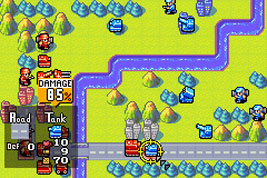
\includegraphics[keepaspectratio]{advance-wars.jpg}
\end{figure}

\begin{figure}[H]
 \caption{A screenshot of Mecho Wars}
 \centering
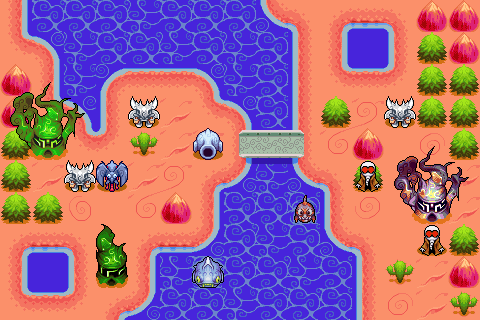
\includegraphics[height=\textheight,width=\textwidth,keepaspectratio]{mecho.png}
\end{figure}

\begin{figure}[H]
 \caption{A screenshot of Battle of Wesnoth}
 \centering
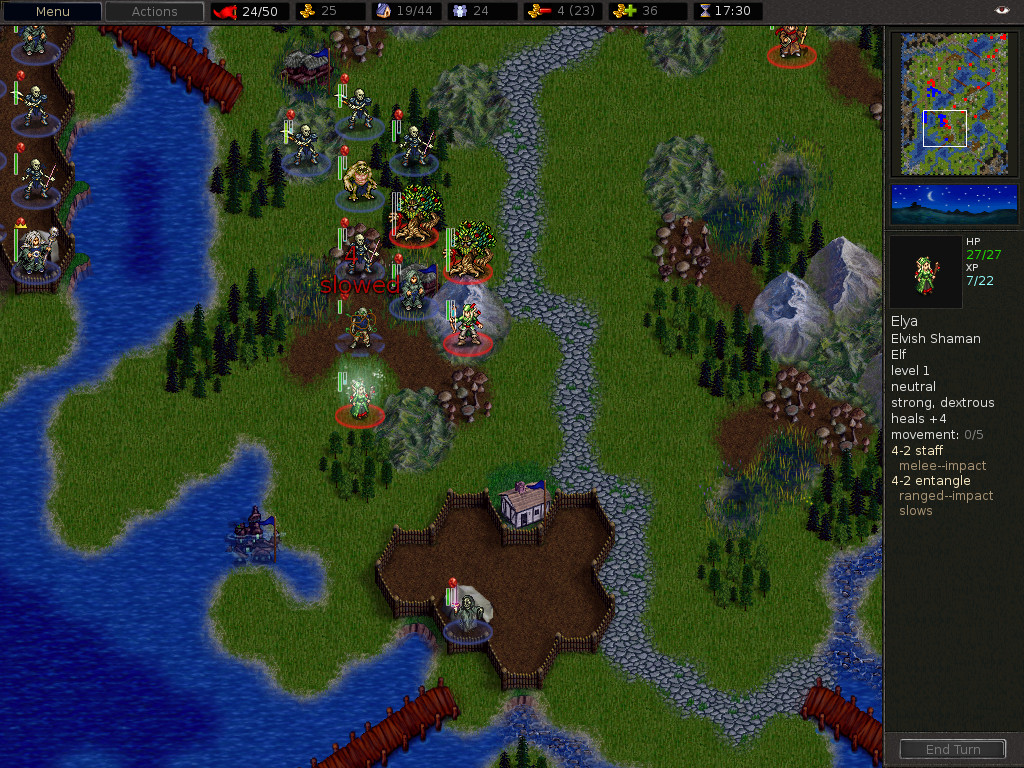
\includegraphics[height=\textheight,width=\textwidth,keepaspectratio]{battle-for-wesnoth-screenshot.jpg}
\end{figure}


\clearpage
\section*{Programme and Methodology}

The overall aim of the project is to work together as a team to produce a turn based strategy game for an android smartphone. This will involve following all of the parts of a software development design life-cycle most likely the waterfall method. The project involves many parts in addition to producing an end product; including researching similar cases and solutions, obtaining the requirements for the system, designing implementing the system, and considering extensibility and maintenance.\\


The game should be intuitive and easy to play and will have an easy to use button based interface. The game should be able to run on any currently available android phone. There will be support for simple multiplayer games either for playing against someone on a different handset or by passing the phone around the players. Due to the scope and time available for the project, multiplayer over different phones may not be viable.  We intend to include a  the ability to store high scores from other  local games  but if we have enough time we would also like to include the ability to store high scores on a server which everyone can view. This would add a more social aspect to the game which is a major advantage for a mobile game.The game graphics will consist of animated colourful sprites with a consistent style. Lots of the features will be based loosely on the game boy advanced game ``Advanced Wars''.\\


The main two options for the development language are C++ and java as the project will be object oriented. The advantages of developing in C++ are smaller memory and CPU footprint which is important for a smart phone. Developing in C++ would be much more of a challenge though as it would require using NDK(Native Development Kit) which would increase the complexity of the program, make the code harder to read and edit later on thus making maintenance harder and also extendibility. Java on the other hand may use more memory and not be as efficient on the CPU but would be significantly easy to develop as the recommended android IDE, ADT(Android Developer Tools) is a full java development IDE. ADT includes the ability to emulate any android device/hardware along with debugging tools specifically for android.\\


By analysing other similar games we hope to further concrete our idea and decide what additional features to add and style to present to the user. We will test lots of similar games and ask potential users what they thought of them in order to determine what it is people what more precisely so we know what to produce. As there is a large number of old games which are similar/have similar concepts, lots of the research will performed by reading reviews on those games and then speaking to people who have played those games to clarify what is was they enjoyed about them and what changes to those games would of made them better. This research can be carried out with questionnaires, interviews and case studies of existing similar games. Because lots of the data we will be collect will be qualitative interviewing people will be essential as it will allow us to prompt them and improve the quality of results, this will help us better define the requirements of the game. Researching into other games with similar ideas will allow us to develop the concept further and to better identify our requirements. This will produce lots of quantitative data which can be analysed and used to create new requirements. The advantage of interviewing people is that they might not be able to effectively convey what it is they liked about other similar old games and what features they would like to see. Collecting information about UI layout from users can be very difficult without being face-to-face and with something physical to show them. By being face-to-face we can get a better idea about how they would like to be able to interact with the game.\\


Because lots of the data we will be collect will be qualitative interviewing people will be essential as it will allow us to prompt them and improve the quality of results, this will help us better define the requirements of the game. Researching into other games with similar ideas will allow us to develop the concept further and to better identify our requirements. This will produce lots of quantitative data which can be analysed and used to create new requirements. The advantage of interviewing people is that they might not be able to effectively convey what it is they liked about other similar old games and what features they would like to see. Collecting information about UI layout from users can be very difficult without being face-to-face and with something physical to show them. By being face-to-face we can get a better idea about how they would like to be able to interact with the game.\\

\subsection*{Collaboration}

Our project will be a collaborative effort of multiple group members working separately on different parts of the system which will then come together to form a finished product. In order to be able to combine parts of the system together into a working entity, all group members need to know what other members are doing. This section isn`t about the interface that will be established during the design stage of the project that we will be able to use to make sure that each part of the system will be able to communicate with another. This section is about collaborating as a team towards a single goal. Being able to see and possibly change each others' work is vital when working as a team. We should also ensure that we use a system which prevents us from overwriting someone elses' work. This is mainly applicable to the programming stage of the project as that's where it is most likely that a member might be wanting to make a change that other members have to be able to see. \\


The solution we have decided to use is the git version control system. Git allows every single member of the group to work on the system locally, making incremental changes. When ready, a group member can push the changes into an online code repository where other group members will be able to see them. The strength of git is the ability to detect when code conflicts occur. If both members change the same part of code, they will be prevented from overwriting the new code without resolving the issue. Furthermore, all users have a copy of the code and can work on it at any time, meaning that they don't have to have network access until the stage where they want to submit the code. Git also features ``branches'' which allow people to work on now concepts or ideas without affecting the main development. As in any version control system, the users are able to roll back the changes to any point in time, meaning that any blunders can be easily reversed. On top of this ability, git is able to make powerful partial reverts, meaning that not all work is lost if we only want to roll back a part of the system. All commits to the system are signed with the commiters name and e-mail address meanining that it's trivial pinpoint who made what changes to the code base.\\

\
As far as the non-programming part of the project goes, regular meetings will be held where group members can discuss any issues they might me having, or any changes they want to make. The work will be split into multiple parts at the beginning of the development life cycle, and those meetings are there to ensure that everyone is keeping up with their work load.\\

All group members have other members' contact details, so we are able to contact any member of the team on individual basis if at all required. We believe that the combination of regular meetings where we can review the progress and the use of a version control system where everyone can see the code is enough to keep the team working efficiently.

\begin{landscape}
\begin{center}
\hspace*{-1.5in}
\vspace*{-1.5in}
\section*{Work plan}
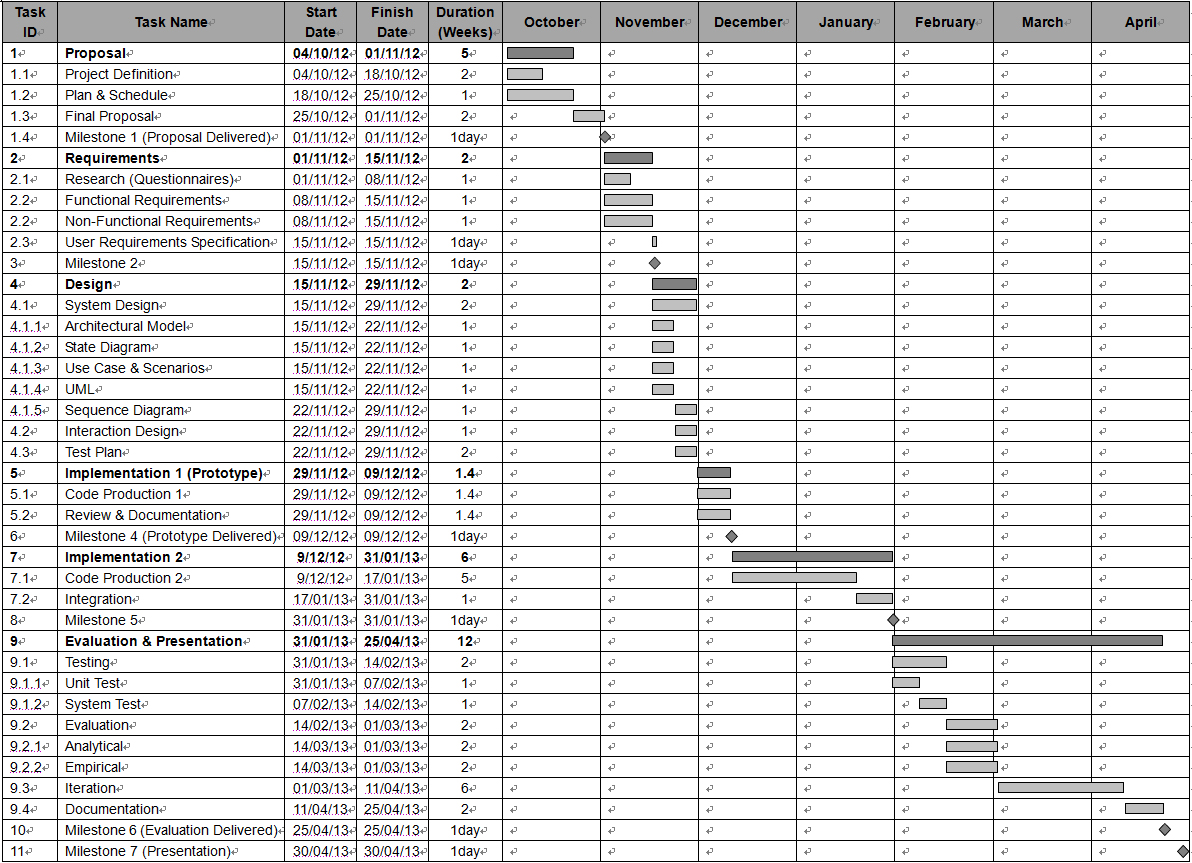
\includegraphics[height=\textheight,keepaspectratio]{gantt.jpg}
\end{center}
\end{landscape}
\end{document}
